\chapter{Modeling}\label{chap:modeling}
We have now introduced the general level set method with curvature- and distance-dependent flow. There were no mentions of how the velocity function should look like to model a curve approximating a set of points, as is the objective of this thesis. Nevertheless, we have seen that if we can describe the desired properties of our curve through an energy function, we can move the curve in the steepest descent direction and thus approach an optimal curve with respect to the defined properties using the gradient flow formulation.

This chapter is about formulating reasonable energy functions and combining the gradient flow theory with the level set method to obtain a complete initial value problem. Given an arbitrary initial curve, the derived models should transform it into a curve approximating given data points while having minimal curvature.

We saw in \secref{sec:shape-derivatives}, that the resulting velocity function \eqref{eq:optimal-descent} is given by the functions $f(\mathbf{x})$ and $g(\mathbf{x})$ and defining these functions is the modeling aspect of the problem. For our situation, we want a curve as close as possible to a set of points while having low curvature. Thus we need to define the functions $f(\mathbf{x})$ and $g(\mathbf{x})$ to be measures of distance and curvature. In general, a minimal curve has the property of having zero mean curvature \cite{meancurv}. Thus we define $g(\mathbf{x})=1$.

We will now introduce three models with different choices of distance-dependent velocity functions $f_p(\distanceVm)$, $p=1,2,3$. The resulting energy function will also 
contain a weighting parameter $\alpha \in [0, 1]$ such that the models can be adjusted depending on how smooth the solution should be. The energy function is defined as
\begin{equation}
    E(\Omega) = \alpha \int_{\Omega} f(d(\mathbf{x}; \pointsetm)) \diff \Omega + (1-\alpha) \int_{\partial \Omega} 1 dS.
\end{equation}
We remember from the introduction to gradient flow, that we want to minimize the energy function. We observe already now that if $f(d(\mathbf{x}; \pointsetm))>0$ for all $\mathbf{x}$, this energy function will have to be positive everywhere and the optimal curve will be the trivial zero solution $\curvem = \partial \Omega = \emptyset$. This is thus something we need to be aware of when constructing appropriate measures of distance $f_p(\distanceVm)$.

Now, as presented in \secref{sec:shape-derivatives}, we minimize the potential energy function using gradient flow, and for that, we need to find the gradient of $E$, $\diff E$. We apply the differentiation formulas \eqref{eq:J1-der} and \eqref{eq:J2-der} from \secref{sec:shape-derivatives} for the two terms of $E$. The resulting derivative is then

\begin{equation}
    \diff E = \int_{\Gamma} \big(\alpha f(d(\mathbf{x}; \pointsetm)) + (1-\alpha)\kappa(u) (\vv{v}(t) \cdot \vv{n}_{\Gamma})\big) \diff S
\end{equation}

Going in the direction of negative directional derivative means moving the curve with speed $\Gamma_t$ defined in \eqref{eq:optimal-descent}, which inserted for $f$ and $g$ is
\begin{equation}
    v_n = (\alpha \, f(d(\mathbf{x};\pointsetm)) + (1-\alpha)\, \kappa(u)).
    \label{eq:general-normal-velocity}
\end{equation}

The resulting level set model for a curve minimizing a function of the distance to a point set while minimizing the mean curvature is thus \eqref{eq:general-normal-velocity} inserted into \eqref{eq:general-level-set}. \\
\newline
\begin{tcolorbox}[title=Generalized level set model]
\begin{equation}
    u_t = |\nabla u|(\alpha \, f(d(\mathbf{x};\pointsetm)) + (1-\alpha)\, \kappa(u)).
    \label{eq:general-model-pde}
\end{equation} 
\end{tcolorbox}

In the following, we will introduce the three distance-dependent functions, and we will for all perform some one-dimensional analysis to get a grasp of the theoretical behavior of the models.






\clearpage
\section{Model 1}\label{sec:model-1}
Model 1 is inspired by a model purposed by Claisse and Frey \cite{Claisse-Frey} which inspired this thesis. They introduced a distance-dependent function that were linearly dependent on an unsigned distance function to the point set. We thus look at a function
\begin{equation*}
    \hat{f}_1(d(\mathbf{x};\pointsetm)) = d(\mathbf{x};\pointsetm).
    \label{eq:pure-dist-model}
\end{equation*}

As stated above, a distance dependent function which is positive everywhere would yield no optimal curve satisfying $\diff E(\Omega) = 0$ except for the trivial zero solution. Also for the attraction term defined above, we see from \eqref{eq:general-normal-velocity} that even when the curve is inside the point set, the velocity would have direction inwards. A natural choice is then to define the distance to be negative inside the point set, thus yielding a curve moving outwards when inside the point set.

This brings us to an interesting question. How do we determine what is on the inside or outside of a set of points? When we discussed the signed distance function, the distance was related a closed curve which has a defined inside. When there is only points, we must be able to draw the boarder between the inside and outside in some way, which means that we must construct a closed curve from the set of points.

We denote the constructed closed curve as $\mathcal{C}_\mathcal{V}$ and thus the signed distance to the curve is $u_d(\mathbf{x}; \mathcal{C}_\mathcal{V})$. Assuming then that we can construct such a curve, we define the distance dependent velocity as 
\begin{equation}
    \tilde{f}_1(d(\mathbf{x};\pointsetm)) = u_d(\mathbf{x}; \mathcal{C}_\mathcal{V}).
    \label{eq:signed-dist-model}
\end{equation}

This may seem like a nice solution. Outside the curve $\mathcal{C}_\mathcal{V}$, the curve, \curve, will be pulled inwards by \eqref{eq:signed-dist-model}, and oppositely it will be pulled outwards if inside $\mathcal{C}_\mathcal{V}$. With no curvature dependent term, we would expect a final curve exactly equal $\mathcal{C}_\mathcal{V}$, and with the curvature term, one could expect a smoother but similar solution. 

The problem is, that we are looking for a curve that can approximate any set of points without assumptions on the structure of the sample points. Without information about the connection between the data points, we can not construct for example a polygon from the data points, which would have been a natural choice. 

Hence, because \eqref{eq:signed-dist-model} do not correspond well with the assumptions for the thesis, we approach the problem differently. With no information about the distribution of points, we go back to the unsigned distance function applied to our point set \distanceV. At all points $\mathbf{x}\in\realspacem^2$, \distanceV\ provides the distance to the closest sampled point in \pointset. Now the speed is decided by the distance to the closest point, and we want to construct a sign function $\sigma(\mathbf{x})$ that determines the direction of the speed in order to pull the curve towards its closest point without making any assumptions on the composition of the data points.

To construct such a sign function, recognize that the only movement we are interested in is the movement of the zero isocontour. Thus the sign function needs only to have a reasonable sign for the values at the zero level curve. We can thus turn the problem around. Rather than figuring out if the curve is inside the point set, we detect whether or not the points in the point set is outside the zero level curve. The curve, \curve, is closed and thus has a meaningful inside and outside. In addition, by construction the sign of \uxt\ is negative inside \curve\ and oppositely positive outside as seen in \eqref{eq:interior}-\eqref{eq:exterior}. 

Using this, we construct the sign function $\sigma(\mathbf{x})$ as follows. For a fixed $t=t^*$, then for every part of the curve $\Gamma(t^*)_r$, denote $\mathbf{v}_r$ as the closest sample point. Then $\sigma(\Gamma(t^*)_r) = \texttt{sgn}(u(\mathbf{v}_r, t^*))$. Because the position of the curve relative to the sample points changes over time, we construct a time dependent sign function that we extend to the entire domain \domain\ as follows:
\begin{equation}
    \sigma(\mathbf{x}, t) = \texttt{sgn}((u(\mathbf{v}_r, t))), \quad \mathbf{v}_r = \texttt{argmin}(\|\mathbf{x}- \mathbf{v}\|_2 \, \forall \mathbf{v} \in \pointsetm). 
    \label{eq:sigma-def}
\end{equation}\todo{figur av sigma som vil se ut som kakestykker}

Using the above, we end up with a model that will draw the curve towards the closest sample points. The distance dependent velocity for model 1 is then defined as
\begin{equation}
    f_1(d(\mathbf{x};\pointsetm)) = \sigma(\mathbf{x}, t) d(\mathbf{x};\pointsetm),
    \label{eq:model1-dist-velocity}
\end{equation}
yielding the full model, by inserting \eqref{eq:model1-dist-velocity} into \eqref{eq:general-model-pde}: \\
\begin{tcolorbox}[title=Model 1]
\begin{equation}
    u_t = |\nabla u|(\alpha\sigma(\mathbf{x}, t) d(\mathbf{x}; \pointsetm) + (1-\alpha) \kappa(x)), \quad \alpha \in \realspacem
    \label{eq:model1-pde}
\end{equation} 
\end{tcolorbox}

\textbf{Remark:} The way $\sigma(\mathbf{x}, t)$ is defined in \eqref{eq:sigma-def} will violate the assumptions in Proposition \ref{prop:shape-derivative} and thus we can not find $\diff E_1$ for this choice of $f(d(\mathbf{x};\pointsetm))$ using the proposition. The sign function makes $f$ discontinuous which makes the velocity discontinuous. This was not mentioned by Claisse and Frey \cite{Claisse-Frey} in their Lemma 2.1, which as we read it must have the same issue. 

As the we will see later, this does not damage the numerical results. The discretized velocity will anyways be discontinuous and thus, as long as the grid size is bounded away from zero, the discontinuity is not detectable. When the grid size is is bigger than some bounding $\epsilon>0$, one can construct a smoothing function, $\tilde{\sigma}$, connecting $\sigma=1$ and $\sigma=-1$ with a bounded derivative which is thus in $L^1$. The resulting velocity will then be continuous and for the discretization, $\sigma=\tilde{\sigma}$. This discrepancy between the theory and the model was found rather late in the process and could be something to look into for further work.


%%%%%%%%%%%%%%%%%%%%%%%%%%%%%%%%%%%%%%
\begin{comment}
We see from \eqref{eq:model1-pde} that the curve will have an inward velocity dependent on the distance to the point set and the curvature. In order to draw the curve towards the point set, the sign function $\sigma$ must be positive when the curve is outside the point set. In that case the distance term is contributing to the inward velocity. 

In the opposite case, when the curve is on the inside, the distance term should contribute to an outward-pointing velocity. This meaning $\sigma(\mathbf{x}, t)$ must be negative. Thus the sign function is clearly defined when the whole curve is outside or inside the point set. When parts of the curve is inside, and other parts are outside of the point set, or when it is hard to define what is outside and inside, this is more complex. 

Claisse and Frey makes no mention of what is done when this is the case, other than that the sign function must be defined locally. Hence, it must be both space and time-dependent. We have made a choice regarding the sign function and decided that the value of the sign function should be dependent on whether or not the closest point in the point set is inside or outside the curve. 

This in practice, means that the curve will always be attracted to the closest point in the point set, which seems like a natural choice because the distance function also is the distance to the same point. 
\end{comment}
\subsection{Radially Symmetric Analysis}
We now reduce the situation down to a radially symmetric setting to perform some simplified analysis of the energy function. The setup can be viewed in \figref{fig:stationary-example}, where we have a circular curve $\Gamma(t)$ with radius \radgamma\ and center in the origin. The point set, \pointset, is also distributed in a circle around the same center and with radius $r_v$. Further more, we assume that the density of the point set is so high that we can approximate the set of point as a continuous curve denoted $\Gamma_{\mathcal{V}}$.

\begin{figure}
    \centering
    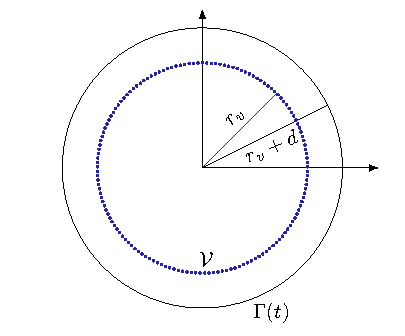
\includegraphics[width=.4\linewidth]{figures/tikz-figures/stationary-example.tex}
    \caption[One dimensional analytical example]{A radially symmetric set up with the point set, $\Gamma_{\pointsetm}$, and curve, $\Gamma (t)$ centered around the origin with radii independent of the angle with respect to the $x$-axis.}
    \label{fig:stationary-example}
\end{figure}
Because of the symmetry and the high density assumption, there will be no spatial discontinuities because the entire curve will either be inside or outside the point set. The resulting \sigmaxt\ will thus be constant in space. Now the energy function $E$ is only a function of \radgamma, and is written
\begin{equation*}
    E(r_{\Gamma}) = \underbrace{\alpha \int_0^{r_{\Gamma}} \texttt{sgn}\{r-r_v\} (r-r_v) 2\pi r \diff r}_\text{$E_1$} + \underbrace{(1-\alpha)\cdot 2\pi r_{\Gamma} \vphantom{ \int_0^{r_{\Gamma}}}}_\text{$E_2$}
\end{equation*}
\begin{equation}
    E(r_{\Gamma}) = \begin{cases}
        2\pi \alpha \bigg( \frac{r_{\Gamma}^3}{3}- \frac{r_{\Gamma}^2 r_v}{2} \bigg) + 2\pi (1-\alpha) r_{\Gamma} &\qquad \text{if } r_{\Gamma}\leq r_v\\
        \frac{2\pi \alpha r_v^3}{3} + 2\pi \alpha \bigg( \frac{r_{\Gamma}^3}{3}- \frac{r_{\Gamma}^2 r_v}{2} \bigg) + (1-\alpha) 2\pi r_{\Gamma} &\qquad \text{if } r_{\Gamma}>r_v
        \end{cases}
    \label{eq:J-rad}
\end{equation}
The total energy function is displayed in \figref{fig:model-jtot} with its separate terms displayed in \figref{fig:model1-j1} for specific parameters $\alpha=0.85$ and $r_v=1$. Here, we see that the energy function does obtain a minimum besides the trivial solution and moreover it is the global minimum. Note also that it is not obtained where $\radgammam=r_v$, but inside the point set, where $\radgammam<r_v$.

\begin{figure}
    \begin{subfigure}[b]{0.48\linewidth}
        \centering
        \includegraphics[width=\linewidth]{figures/Model-1/Jis.tex}
        \caption{The separate energy terms}
        \label{fig:model1-j1}
    \end{subfigure}
    \begin{subfigure}[b]{0.48\linewidth}
        \centering
        \includegraphics[width=\linewidth]{figures/Model-1/J.tex}
        \caption{Total energy function}
        \label{fig:model-jtot}
    \end{subfigure}
    \caption[Minimization problem]{The potential energy function for model 1 \eqref{eq:J-rad} in the radially symmetric situation with $\alpha=0.85$ and $r_v=1$}
    \label{fig:minimization-model1}
\end{figure}

We stick to this radially symmetric situation, and we will see that in one dimensions, \eqref{eq:general-model-pde} is a hyperbolic conservation law.

\subsection*{Method of characteristics}
A scalar hyperbolic conservation is a PDE that can be written in the form 
\begin{equation}
    u_t + \diff f(u) \nabla u = 0,
    \label{eq:general-hyp-cons}
\end{equation}
where $f=(f_1,\dots, f_m)$ and $x=(x_1, \dots, x_n)$\cite{MR3443431}. This can not be done for \eqref{eq:model1-pde} which defines our model in the two-dimensional case because the curvature term is parabolic. However, in the one-dimensional case the curvature reduces to
\begin{equation*}
    \nabla \cdot \frac{\nabla u}{|\nabla u|} = \bigg( \frac{u_x}{|u_x|} \bigg)_x = (\pm 1)_x = 0.
\end{equation*}
We immediately get that \eqref{eq:model1-pde} turns into
\begin{equation*}
    u_t = \pm u_x \alpha \sigma(x) d(x; \pointsetm),
\end{equation*}
which for a $\diff f(u) = \mp \alpha \sigma d(x; \pointsetm)$ is a hyperbolic conservation law as in \eqref{eq:general-hyp-cons}. Because the curvature term is meaningless in one dimensions, this is less interesting seen as it is a key feature for our model. 

In a radially symmetric situation, the curvature is more interesting. The setup is the same as in the calculations leading up to \eqref{eq:J-rad} an is shown in \figref{fig:stationary-example}. For both \pointset\ and $\Gamma$ being circles with the same center, the distance $d(r; \pointsetm) = |r-r_v|$ and the curvature of a circle is known as
\begin{equation}
    \kappa(r) = \frac{1}{r}
    \label{eq:curvature-circle}
\end{equation}
\begin{comment}
\subsection{1 spatial dimension}
\begin{figure}
    \centering
    \includegraphics{figures/tikz-figures/characteristics-1d-initial.tex}
    \caption[Method of characteristics - initial function]{Caption}
    \label{fig:1d-char}
\end{figure}

We look at our equation \todo{ref} in one dimensions. The situation is as pictured in \figref{fig:1d-char}, with the point set consisting of two points, $\mathcal{V}=\{v_1, v_2\}$. We can then assume without loss of generality that they are placed symmetric around the origin. First of all, we notice that in one dimensions, the notion of curvature is meaningless.
\begin{equation}
    \kappa(u) = \Bigg( \frac{u_x}{|u_x|} \Bigg)_x = (\pm 1)_x = 0
\end{equation}

We then have that our level set equation simply is
\begin{equation}
    u_t =\alpha \sigma (x) d(x)\, u_x
\end{equation}

Because our problem is symmetric, the function, $\sigma (x) = \pm 1$, depending on our initial function has a level set that is inside or outside the point set. 

\end{comment}
The term $|\nabla u|$ can be expressed in terms of $r$ through a simple change of variables:
\begin{align*}
    r &=\sqrt{x^2+y^2} \\
    \implies \frac{dr}{dx} &= \frac{x}{\sqrt{x^2 + y^2}} \\
    \implies \frac{dr}{dy} &= \frac{y}{\sqrt{x^2+ y^2}} \\
    |\nabla u| &= \sqrt{u_x^2 + u_y^2} = \sqrt{\frac{\partial u}{\partial r} \frac{dr}{dx} + \frac{\partial u}{\partial r} \frac{dr}{dy}}
\end{align*}
\begin{equation}
    \implies |\nabla u | = \sqrt{\frac{u_r^2}{x^2+y^2} (x^2 + y^2)} = u_r, \qquad \text{if } u_r\geq 0
    \label{eq:nablau-ur}
\end{equation}

Inserting \eqref{eq:curvature-circle} and \eqref{eq:nablau-ur} into \eqref{eq:model1-pde} we get
\begin{equation}
    u_t = u_r \bigg(\alpha \sigma(t)|r-r_v| + \frac{(1-\alpha)}{r} \bigg).
    \label{eq:zero-levelset-polar-coords}
\end{equation}

We have now a conservation law on the form \eqref{eq:general-hyp-cons} for $r$. Because our PDE now is only dependent on the radius, the total derivative of \eqref{eq:zero-levelset-polar-coords} with respect to time becomes
\begin{equation}
    \frac{du}{dt} = u_t + u_r \,r_t.
    \label{eq:polar-characteristic-eq}
\end{equation}

We want to investigate how the curve moves in time. The curve is always the zero level set, and is thus by definition constant and equal to zero. Moreover, the PDE can be even simplified further at the curve because we have that $\sigma(t)(|r_{\Gamma}-r_v|) = (r_{\Gamma}-r_v)$ at the curve, since the sign function changes at the point when $r_{\Gamma}=r_v$. Thus 
\begin{equation}
    u_t = u_r \bigg(\alpha (r-r_v) + \frac{(1-\alpha)}{r} \bigg) \qquad \text{for } r=\radgammam.
    \label{eq:levelset-polar-coords}
\end{equation}
Because of the constant value for $u$ at all level curves, the left hand side in \eqref{eq:polar-characteristic-eq} equals zero. And thus
\begin{equation}
    u_t=-u_r\, r_t,
    \label{eq:characteristic-streamline}
\end{equation}
and by comparing \eqref{eq:characteristic-streamline} with \eqref{eq:zero-levelset-polar-coords}, we see that
\begin{equation}
    r_t = -\bigg(\alpha \sigma|r(t)-r_v| + \frac{(1-\alpha)}{r(t)}\bigg),
    \label{eq:pde-streamline}
\end{equation}
where $r(t)$ is the radius for a single iso-contour which moves in time. We will call the trajectories of the curves following \eqref{eq:pde-streamline}, the streamlines for the solution. First, we want to analyze how the zero level curve moves given an initial radius, $r_0$. We then compare  \eqref{eq:levelset-polar-coords} and \eqref{eq:zero-levelset-polar-coords} to obtain the PDE for the streamline of a zero iso-contour
\begin{equation}
    r_t = -\bigg(\alpha (r(t)-r_v) + \frac{(1-\alpha)}{r(t)}\bigg) \quad \text{for }r(t) = r_{\Gamma}.
    \label{eq:pde-zero-streamline}
\end{equation}

The equation \eqref{eq:pde-zero-streamline} is a separable equation, and the solution is an implicit function of $r(t)$,
\begin{equation}
    \frac{\ln(\alpha(r(t)^2-r_v\,r(t)-1)+1) - \frac{2\sqrt{\alpha}\,r_v \tan^{-1}\bigg(\frac{\sqrt{\alpha} (r_v-2r(t))}{\sqrt{4-\alpha(r_v^2+4)}}\bigg)}{\sqrt{4-\alpha(r_v^2+4)}}}{2\alpha}=-t+C,
    \label{eq:streamline-solution}
\end{equation}
where the constant $C$ is decided from the initial conditions, $t=0$, $r=r_0$.
\begin{equation}
    C=\frac{\ln(\alpha(r_0^2-r_v r_0-1)+1) - \frac{2\sqrt{\alpha}\,r_v \tan^{-1}\bigg(\frac{\sqrt{\alpha} (r_v-2r_0)}{\sqrt{4-\alpha(r_v^2+4)}}\bigg)}{\sqrt{4-\alpha(r_v^2+4)}}}{2\alpha}.
    \label{eq:streamline-solution-constant}
\end{equation}

\begin{figure}
    \begin{subfigure}[b]{0.48\linewidth}
    \centering
        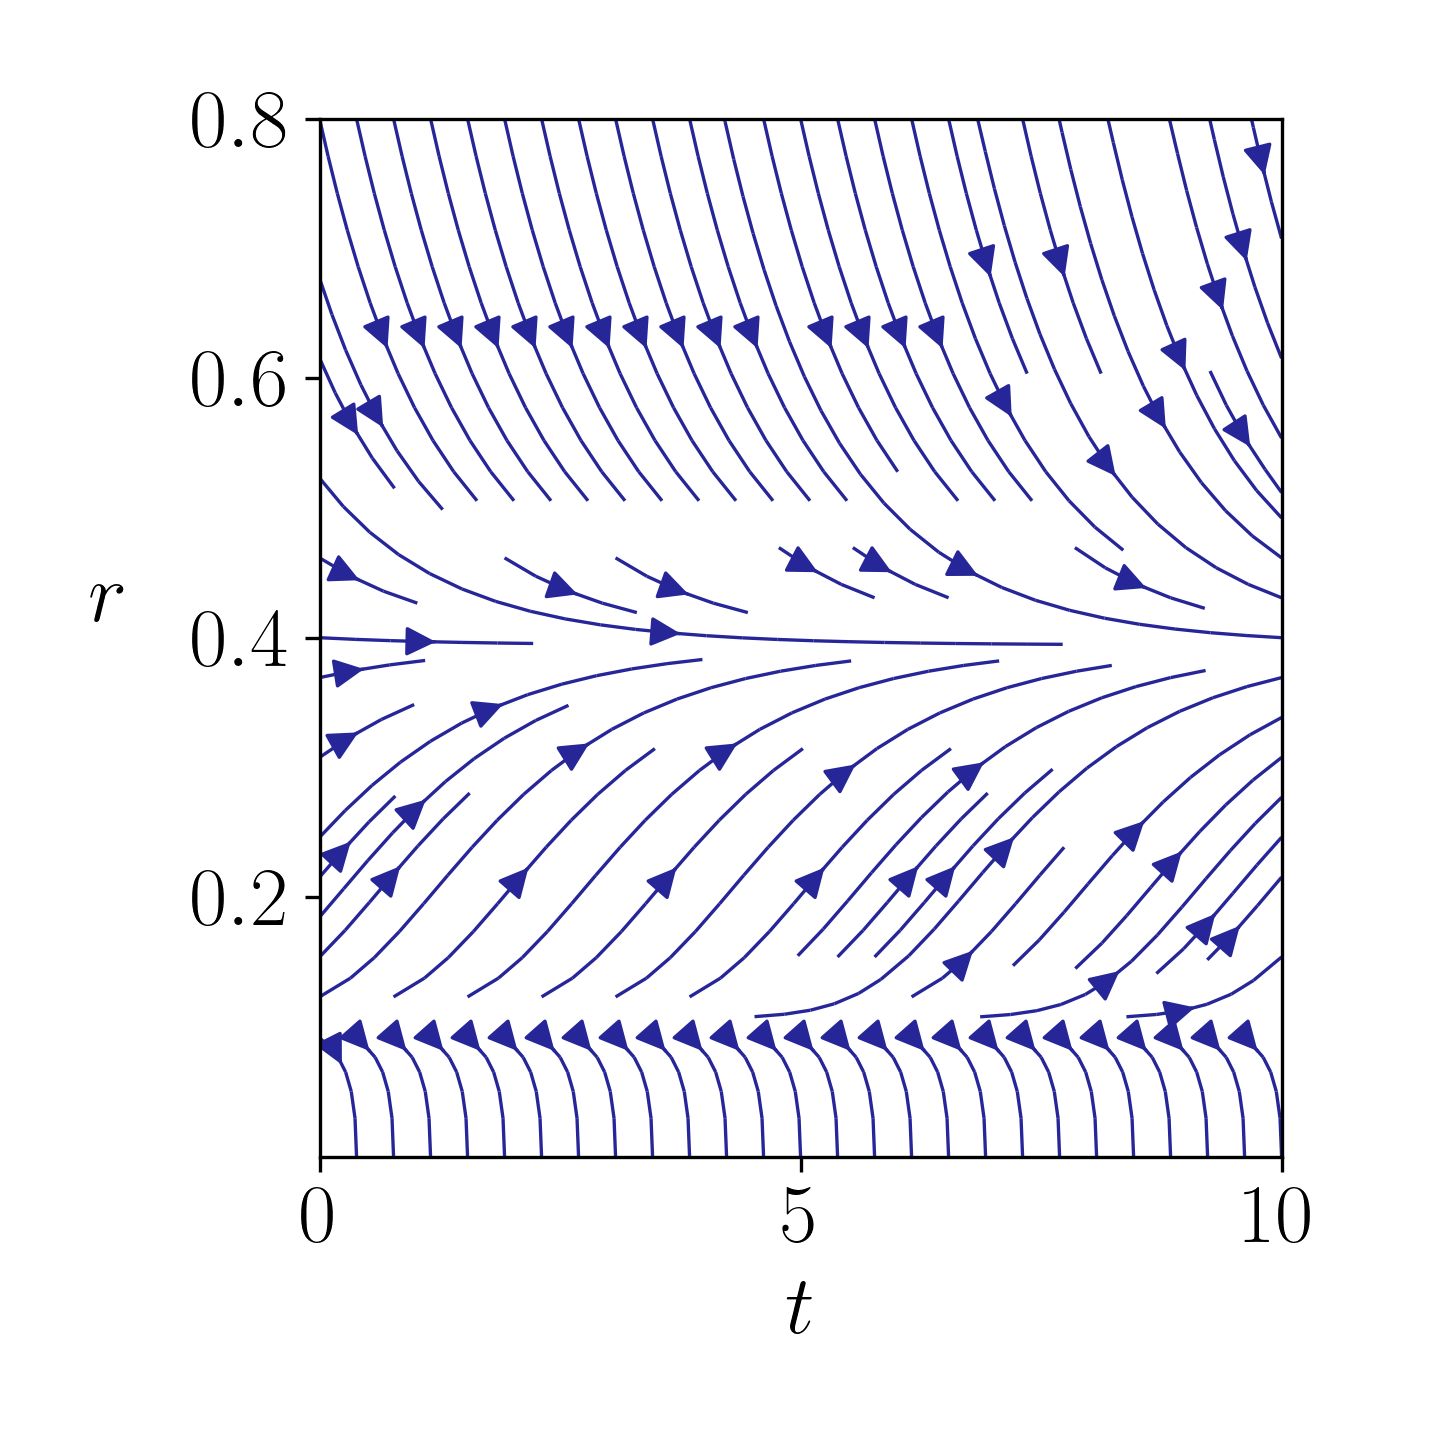
\includegraphics[width=\linewidth]{figures/streamlines/mod1-a96.png}
        \caption{$\alpha=0.96$} 
        \label{fig:radius-characteristics-96} 
    \end{subfigure}
    \begin{subfigure}[b]{0.48\linewidth}
    \centering
        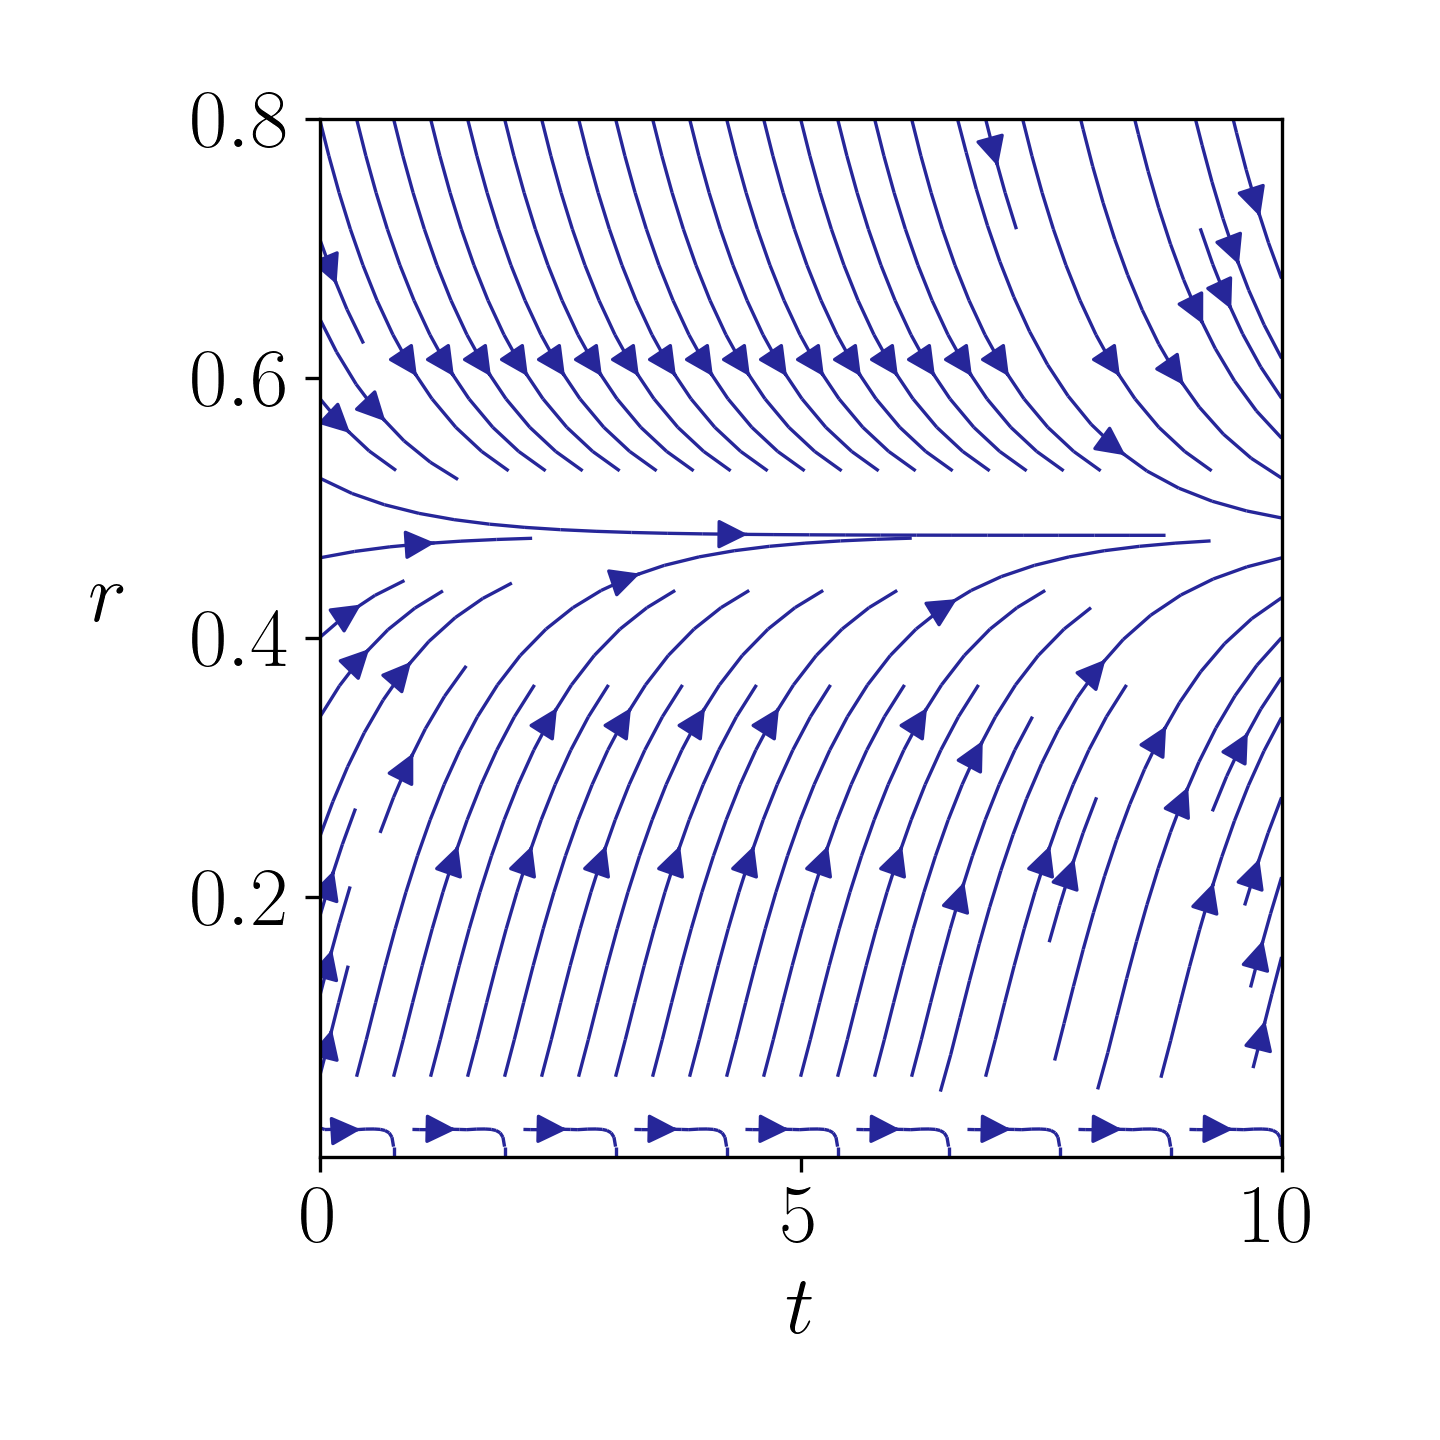
\includegraphics[width=\linewidth]{figures/streamlines/mod1-a99.png}
        \caption{$\alpha=0.99$} 
        \label{fig:radius-characteristics-99} 
    \end{subfigure} 
    \caption[Streamlines in the radially symmetric situation]{Streamlines for the zero level set curve, $\Gamma(t)$, in the radially symmetric situation with the pointset, \pointset, situated at $r_v=0.5$.}
    \label{fig:radius-characteristics}
\end{figure}

The motion of the streamlines can also be viewed in \figref{fig:radius-characteristics}, where we can follow the radius of the zero level set curves starting at a given radius, $r_0$.

We can also construct a general characteristic field for a situation with a fixed $\alpha$, point set radius $r_v$ and initial radius, $r_0$ by solving \eqref{eq:pde-streamline}. First we look at the term $\sigma(t) d(r)$ given the radius of the zero level set curve $r_{\Gamma}$
\begin{alignat}{3}
    \sigma(r_{\Gamma}, t)d(r) &= &|r-r_v| \qquad & \text{when }\radgammam \geq r_v \label{eq:sigma-radius-1}\\
    \sigma(r_{\Gamma}, t)d(r) &= -&|r-r_v| \qquad & \text{when }\radgammam < r_v \label{eq:sigma-radius-2}
\end{alignat}
Thus we can write \eqref{eq:pde-streamline} in terms of $r_\Gamma$ as
\begin{alignat}{3}
    r_t &= -&\bigg(\alpha |r(t)-r_v| + \frac{1-\alpha}{r(t)}\bigg) \qquad &\text{when }\radgammam \geq r_v \\
    r_t &= &\bigg(\alpha |r(t)-r_v| -  \frac{1-\alpha}{r(t)}\bigg) \qquad &\text{when }\radgammam < r_v,
\end{alignat}
Thus, the only thing we need in order to make the full characteristic field is to find the time when $r_{\Gamma} = r_v$, which can be found from \eqref{eq:streamline-solution} and \eqref{eq:streamline-solution-constant}.

This is done in \figref{fig:total-streamline-picture} for a curve starting with $r_0=0.6$ with a point set, $\mathcal{V}$, situated in $r_v=0.5$ and the weighting $\alpha = 0.96$. A useful formula when $(4-\alpha(r_v^2+4))<0$, which is also true for this case, is that the arctangent of an imaginary number is
\begin{equation*}
    \tan^{-1}(i x ) = \frac{i}{2} \ln\bigg(\frac{1+x}{1-x} \bigg).
\end{equation*}

In the figure, we see that the streamlines stemming from the area around the initial curve moves similarily to the zero iso-contours in \figref{fig:radius-characteristics-96}, but further away, they differ more and more. That is because the sign change of $\sigma(r, t)$ happens more and more out of sync with when that particular level set falls into the point set. 

We also observe in the \figref{fig:total-streamline-picture} that level curves in a band around the zero level curve approaches the stationary radius as well. When numerous level curves approach the same radius, the higher dimensional function becomes steeper and steeper. This can cause problems for a numerical scheme which is sensitive to steep gradients.


\begin{figure}
    \begin{subfigure}{.5\linewidth}
        \centering
        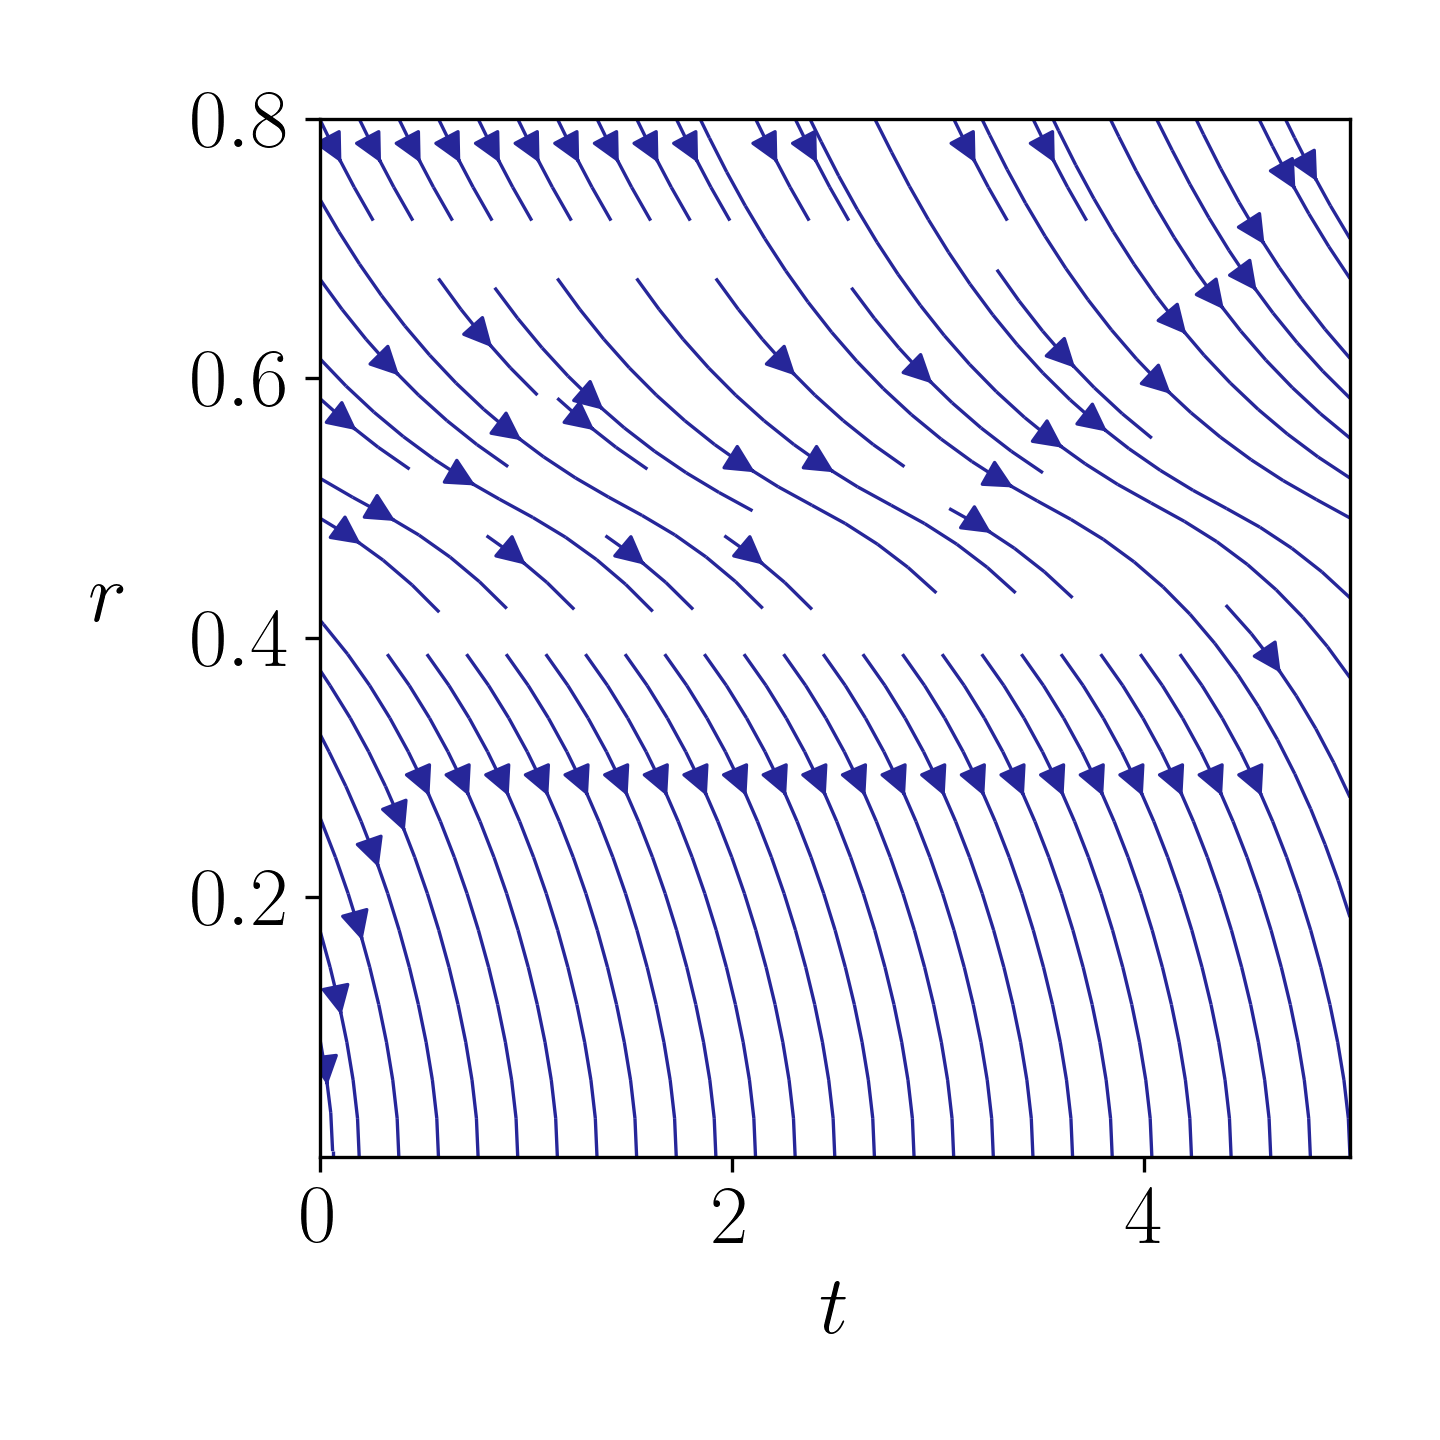
\includegraphics[width=\linewidth]{figures/streamlines/mod1-a96-pos.png}
        \caption{Streamlines with $\sigma(r, t) = 1$}
        \label{fig:sub1}
        \end{subfigure}%
    \begin{subfigure}{.5\linewidth}
        \centering
        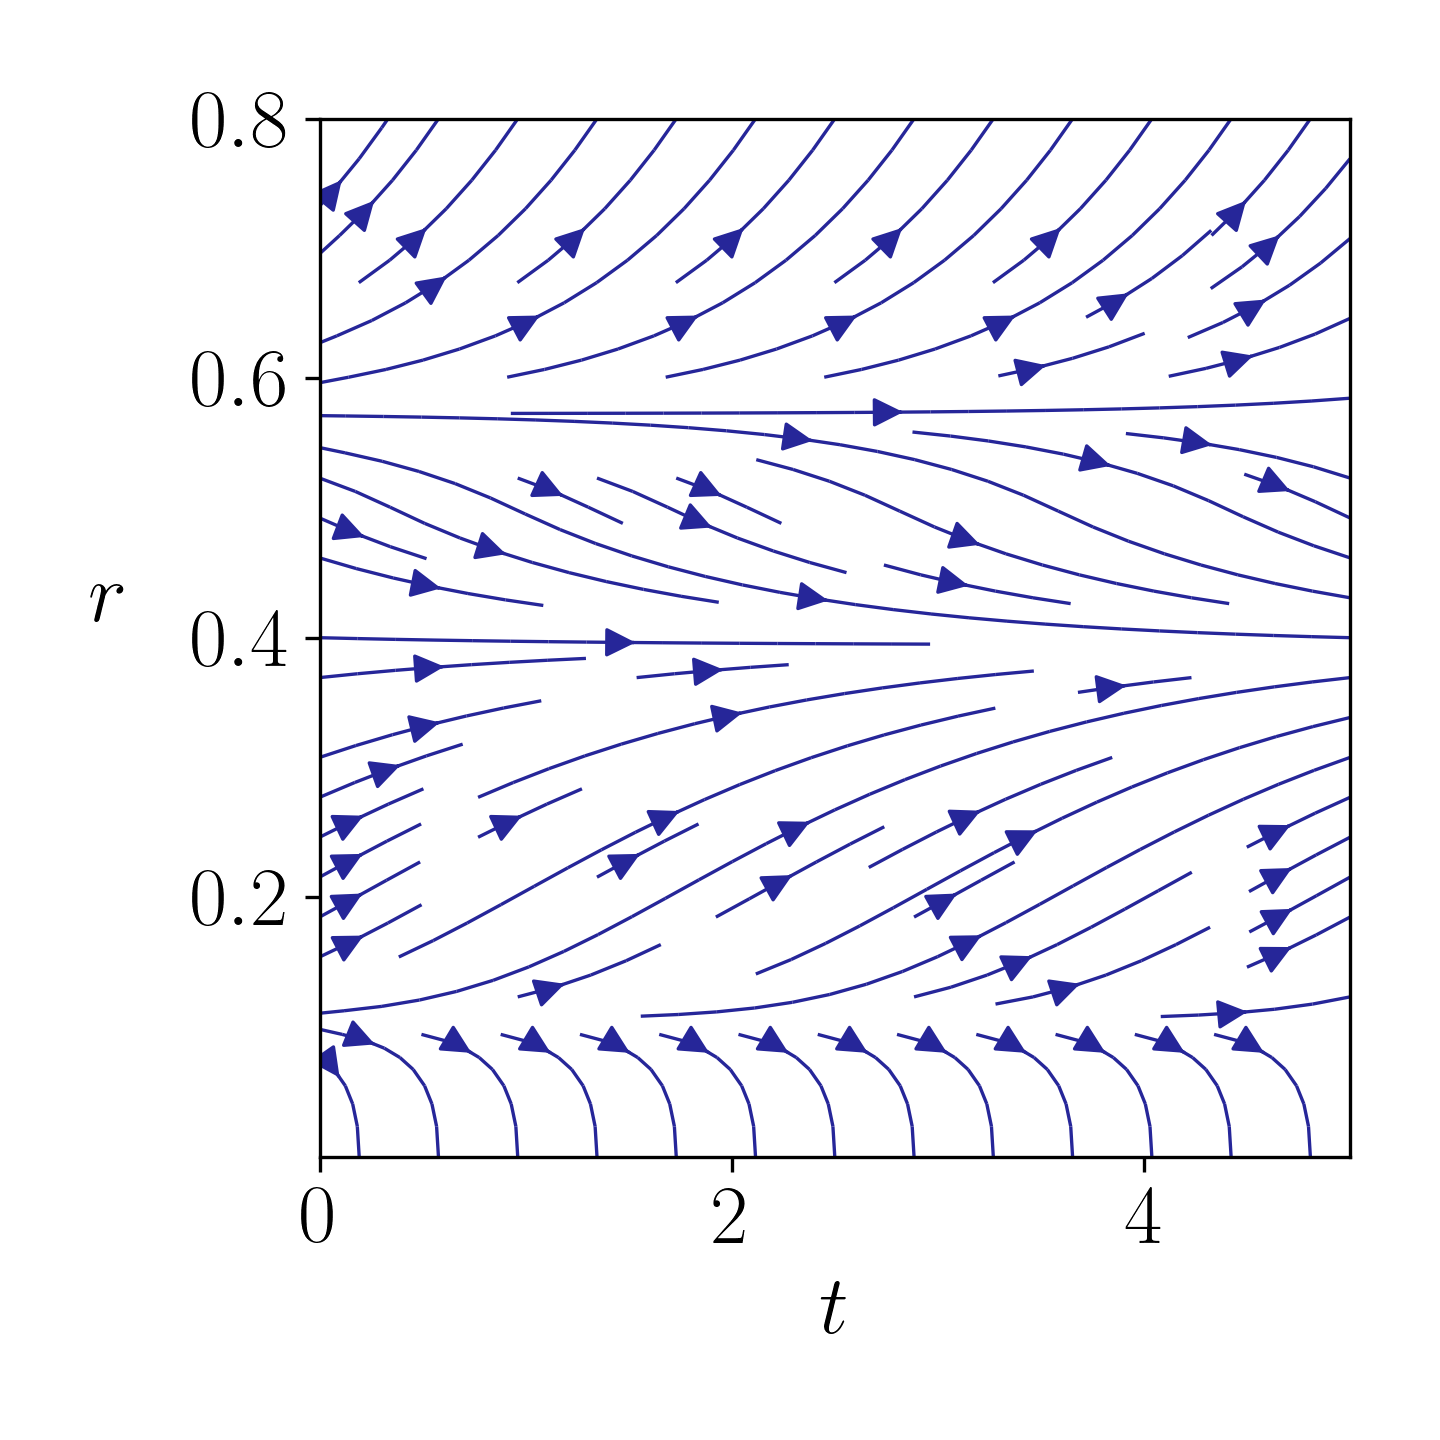
\includegraphics[width=\linewidth]{figures/streamlines/mod1-a96-neg.png}
        \caption{Streamlines when $\sigma(r, t)=-1$}
        \label{fig:sub2}
        \end{subfigure}\\[1ex]
    \begin{subfigure}{\linewidth}
        \centering
        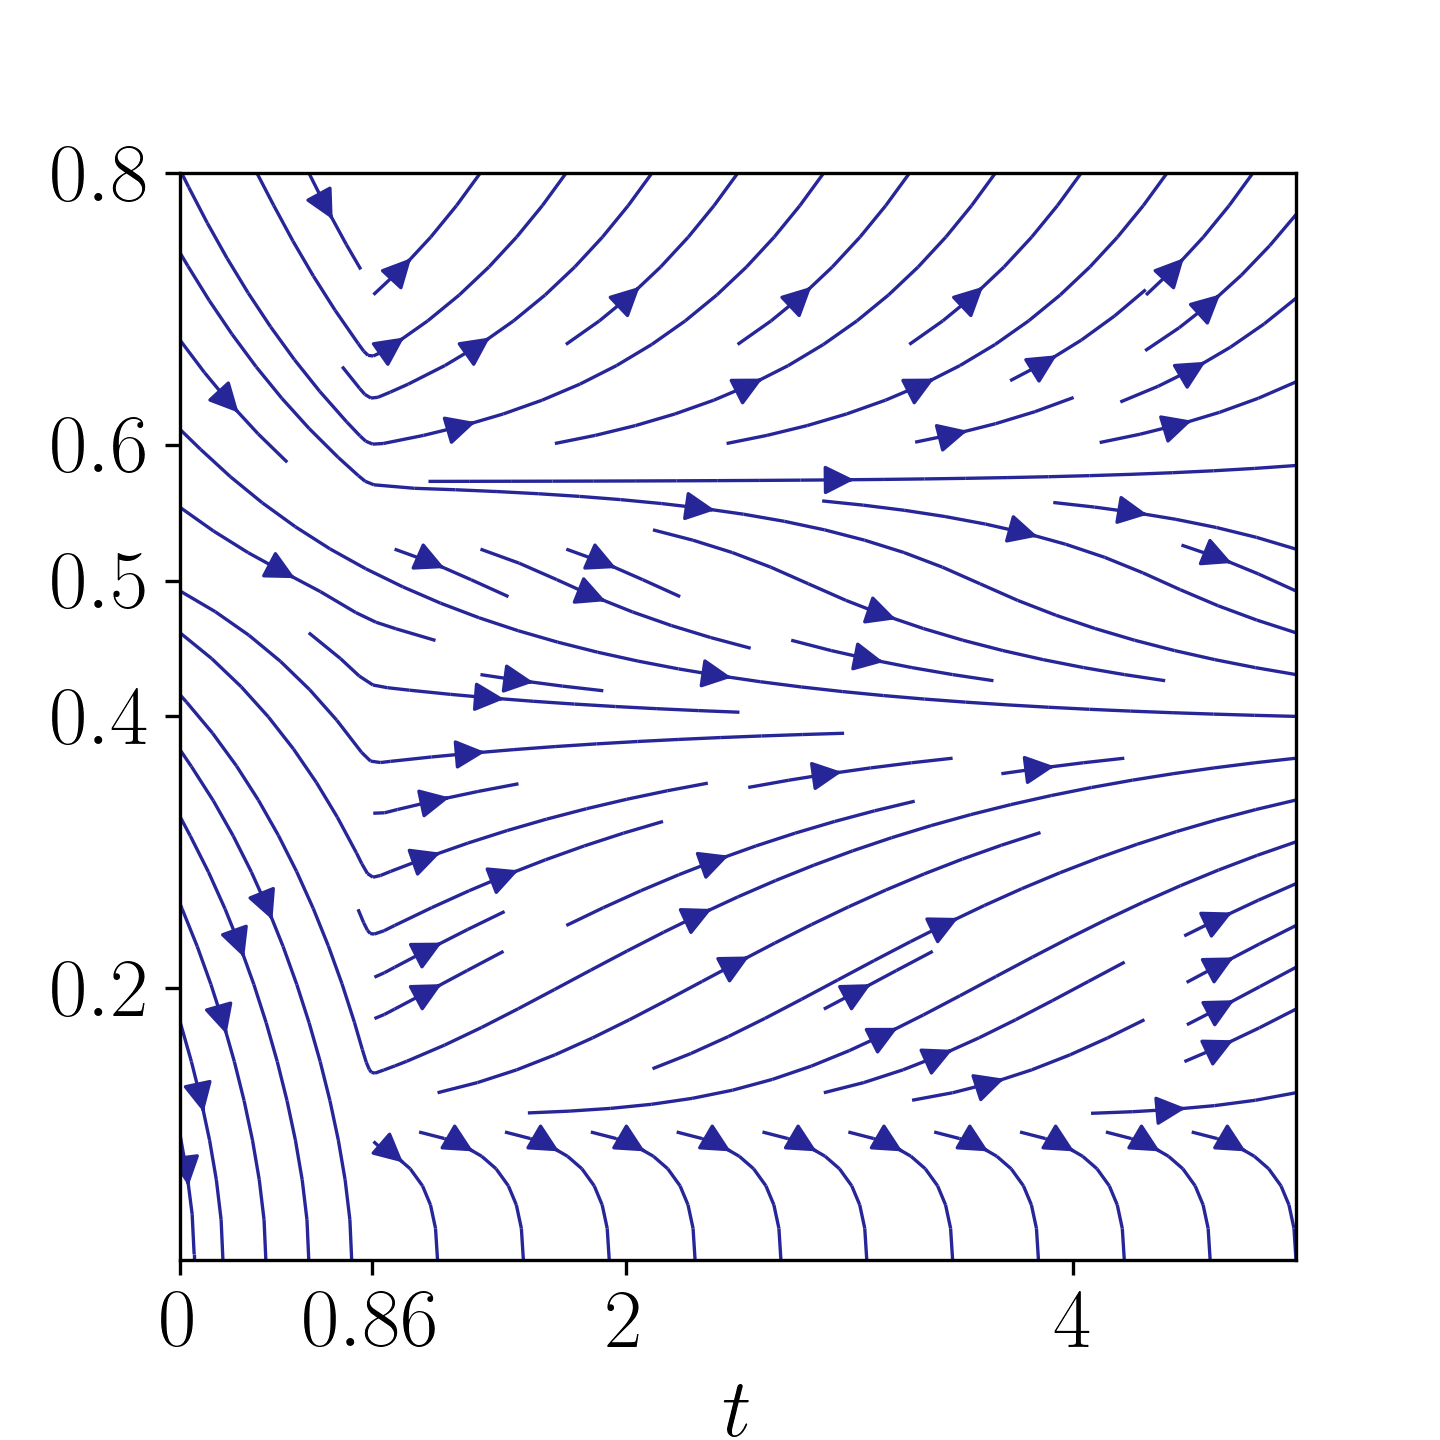
\includegraphics[width=.5\linewidth]{figures/streamlines/mod1-a96-tot.png}
        \caption{Streamlines for all level curves when the zero level set curve, $\Gamma (t)$ has initial radius, $r_0=0.6$.}
        \label{fig:sub3}
    \end{subfigure}
    \caption[Streamlines for all level curves]{Streamlines when the sign function is $\sigma(r, t) = +1$ and $\sigma(r, t) = -1$, for a point set with radius, $r_v=0.5$ and weight $\alpha=0.96$ on top. The lowermost figure shows the streamlines when the zero level set curve has initial radius $r_0=0.6$. Meaning that the sign of $\sigma(r, t)$ changes in $t=0.86$.}
    \label{fig:total-streamline-picture}
\end{figure}




\subsection*{Stationary solutions}
We now want to examine stationary solutions for \eqref{eq:zero-levelset-polar-coords}. In the context of level set methods, the stationary solution is obtained when the zero level curve is stationary. See for example in \figref{fig:total-streamline-picture} that when the zero level curve converges, the iso-curves above a certain value diverges. The stationary zero level curve can be obtained by finding the minima of $E(\Omega)$ or in the radially symmetric situation---finding $r_f = \lim_{t\to\infty} r(t)$ given an initial radius, $r_0$ or in other words when $r_t=0$ in \eqref{eq:pde-zero-streamline}.

We can observe in \figref{fig:radius-characteristics} that the stationary radius, $r_f$ for the zero level curve depends on the weighting $\alpha$, when $\alpha$ increased, the stationary radius was much closer to the radius of the point set. We will now find the exact relation.

We set $r_t$ in \eqref{eq:pde-zero-streamline} equal zero and denote the radius where this is fulfilled as $r_f$. We solve for $r_f$ and obtain  
\begin{equation}
    0 = \alpha (r_f-r_v) + \frac{1-\alpha}{r_f}.
    \label{eq:steady-state-circle}
\end{equation}

We multiply \eqref{eq:steady-state-circle} with $r_f/\alpha$ and obtain a quadratic equation
\begin{equation*}
    r_f^2-r_v\, r_f+ \frac{1-\alpha}{\alpha} = 0,
\end{equation*}
which has the solution
\begin{equation}
    r_f = \frac{r_v}{2} \pm \frac{\sqrt{r_v^2-4 (1-\alpha)/\alpha}}{2}.
    \label{eq:stationary-radius}
\end{equation}

First of all, we see that with $\alpha=1$, $r_f=r_v$. Setting $\alpha=1$ is equal to a velocity field that is only distance dependent, and then it is as we expect that the curve ends up covering the point set, unaffected by curvature. We also see immediately that there are two solutions, meaning two stationary radii, which is located at both sides of $r=r_v/2$. This is also what we observe in \figref{fig:radius-characteristics}. Note also that only one of the stationary solutions, namely the outermost of the two, is stable, and that the innermost is only the point where the curvature exceeds the distance function and pulls it inwards to zero radius. \todo{Bevis påstand om ustabil indre løsning}

What we also get from \eqref{eq:stationary-radius} is that we can find the minimal $\alpha$ for which we can obtain a stationary solution at all. When 
\begin{equation*}
    r_v^2 < \frac{4(1-\alpha)}{\alpha},
\end{equation*}
there will be no real solution to \eqref{eq:stationary-radius}. Solving for $\alpha$ gives a restriction for the weighting parameter being
\begin{equation}
    \alpha \geq \frac{4}{r_v^2 + 4}.
    \label{eq:weighting-restriction}
\end{equation}

When $\alpha$ does not fulfill \eqref{eq:weighting-restriction}, the zero level curve will have a velocity driven mostly by the curvature and with constant direction inwards, which will drive the radius smaller and smaller until the circle disappears.

An important result, which we take from this analysis is that when \\ $\alpha<1$, which means whenever the curvature also influences the motion, the stationary solution for the curve will always be inside the point set for a dense circle. The distance is given by $d(r_f) = |r_f-r_v|$ and inserting $r_f$ from \eqref{eq:stationary-radius}. This can also be observed directly from our velocity function \eqref{eq:general-normal-velocity}, because when the curve covers our point set, the distance function is zero, but $\kappa(r) = 1/r_v\neq 0$, which means that the curve still has speed inwards. 

The stationary solution is thus the point where the distance and curvature is balanced, meaning that the stationary solution is not bound to cover the point set nor ensure zero curvature at the stationary solution. Thus we do not minimize both the curvature and distance, but we get a weighting of the two. We thus get a curve that will have low curvature close to the point set and high curvature far away.



% NB When I tested for a = 0.96, rv=0.5 I got r=0.3757 in stead of 0.4!! This was for h=1/100



\section{Model 2}
As seen from the analysis above for the first model, the stationary solution for a circle of dense points would not approach the point set except for $\alpha=1$. Also, if the point set was not as dense, the curvature would be low near the points and conversely high far away.

The idea behind model 2 is to aim for the opposite, meaning a curve with high curvature near the points and approaching straight lines further away. This will be more similar to smoothed polygons with the sampled points as edges. 

In order to do so, the distance dependent function $f_2(d(\mathbf{x}; V)$ is chosen to be inversely proportional to the distance, and thus defined as
\begin{equation}
    f_2(d(\mathbf{x}; V) = \frac{\sigma(\mathbf{x}, t)}{\beta d(\mathbf{x})+\delta},
    \label{eq:f-2}
\end{equation}
Hence $f_2(d(\mathbf{x}; V)$ will be large close to the point set yielding a stationary solution of high curvature. Furthermore, the distance-dependent term in the energy function will be similar to a gravitational field, attracting more and more the closer to the source. The resulting model is obtained by inserting \eqref{eq:f-2} into \eqref{eq:general-model-pde}.

\begin{tcolorbox}[title=Model 2]
\begin{equation}
    u_t = |\nabla u| \bigg(\alpha \frac{ \sigma(\mathbf{x}, t)}{\beta d(\mathbf{x})+\delta} + (1-\alpha)\kappa (u) \bigg), \qquad \alpha, \beta, \delta \in \realspacem
    \label{eq:model2-pde}
\end{equation}
\end{tcolorbox}
Where the parameter $\delta>0$ avoids the velocity having a singularity at points in the point set and the term $\beta>0$ is a scaling parameter. Without varying the parameter $\beta$ with the domain size, identical point sets of different scalings will yield different curves.

\subsection{Radially Symmetric Analysis}
We conduct the same analysis for model 2 as for model 1. Using \eqref{eq:curvature-circle} and \eqref{eq:nablau-ur} and that $d(r)=|r-r_v|$, we obtain a radially dependent normal velocity
\begin{equation}
    v_n = \frac{\alpha \sigma(r_{\Gamma}, t)}{\beta (|r-r_v|)+\delta} + \frac{1-\alpha}{r}.
    \label{eq:general-inverse-velocityfield}
\end{equation}
Following the procedure for model 1 further, we find that the ODE for the characteristics/streamlines for the level curves is defined by $r_t = -v_n$ and using \eqref{eq:sigma-radius-1}-\eqref{eq:sigma-radius-2} to rewrite $\sigma(r, t)$ and inserting into \eqref{eq:general-inverse-velocityfield} we get the velocity for all level curves with a radius $r(t)$, as 
\begin{alignat}{3}
    r_t &= -&\bigg(\frac{\alpha }{\beta(|r(t)-r_v|)+\delta} + \frac{1-\alpha}{r(t)}\bigg) \qquad &\text{if }r_{\Gamma} \geq r_v,\\
    r_t &= &\bigg(\frac{\alpha}{\beta(|r(t)-r_v|)+\delta} -  \frac{1-\alpha}{r(t)}\bigg) \qquad &\text{if }r_{\Gamma} < r_v.
\end{alignat}

Because we add the small constant $\delta$ to the denominator in \eqref{eq:general-inverse-velocityfield} we cannot in the same manner as for \eqref{eq:pde-zero-streamline} remove the absolute value for the zero level curve because the sign of $\delta$ should also be changed when $r(t)=r_v$. For the zero level curve, we then get the set of equations which applies for the two cases when the curve is outside or inside the point set.
\begin{alignat}{3}
    r_t &= -&\bigg(\frac{\alpha}{\beta(r(t)-r_v)+\delta} + \frac{(1-\alpha)}{r(t)}\bigg) \quad &\text{for }r(t) = r_{\Gamma}>r_v, \label{eq:pde-zero-streamline-inverse-1} \\
    r_t &= &\bigg(\frac{\alpha}{\beta(r_v - r(t))+\delta} -  \frac{(1-\alpha)}{r(t)}\bigg) \quad &\text{for }r(t) = r_{\Gamma}>r_v.\label{eq:pde-zero-streamline-inverse-2}
\end{alignat}
    

Thus, solving \eqref{eq:pde-zero-streamline-inverse-1} and \eqref{eq:pde-zero-streamline-inverse-2} with $r_t=0$ gives the stationary solution, $r_f$. We begin with \eqref{eq:pde-zero-streamline-inverse-1} which yields  
\begin{equation*}
\begin{cases}
    r_f = \frac{\beta (1-\alpha)}{\alpha + \beta (1-\alpha)} (r_v-\delta/\beta), \\
    r_f > r_v.
\end{cases}
\end{equation*}
We see that for all choices of $\alpha \in [0, 1]$, $\delta>0$ and $\beta>0$, $r_f$ will have to be smaller than $r_v$. This does not satisfy the constraint $r_f>r_v$, and thus the stationary solution of \eqref{eq:pde-zero-streamline-inverse-1} is not feasible. We proceed to look at the situation where $r_{\Gamma}<r_v$ in \eqref{eq:pde-zero-streamline-inverse-2} which has the stationary solution
\begin{equation}
\begin{cases}
    r_f = \frac{\beta (1-\alpha)}{\alpha + \beta (1-\alpha)} (r_v+\delta/\beta), \\
    r_f < r_v.
\end{cases}
\label{eq:stationary-sol-inverse}
\end{equation}
Neither for \eqref{eq:stationary-sol-inverse}, the stationary radius is guaranteed to exist but depends in the parameter choices. Furthermore, we see that we can make $r_f \sim r_v$ by choosing $\delta$ small and $\alpha$ big, but we see in \figref{fig:total-streamline-inverse} that this solution is unstable. \todo{Vis at stasjonær løsning ustabil}

\begin{figure}
    \begin{subfigure}{.5\linewidth}
        \centering
        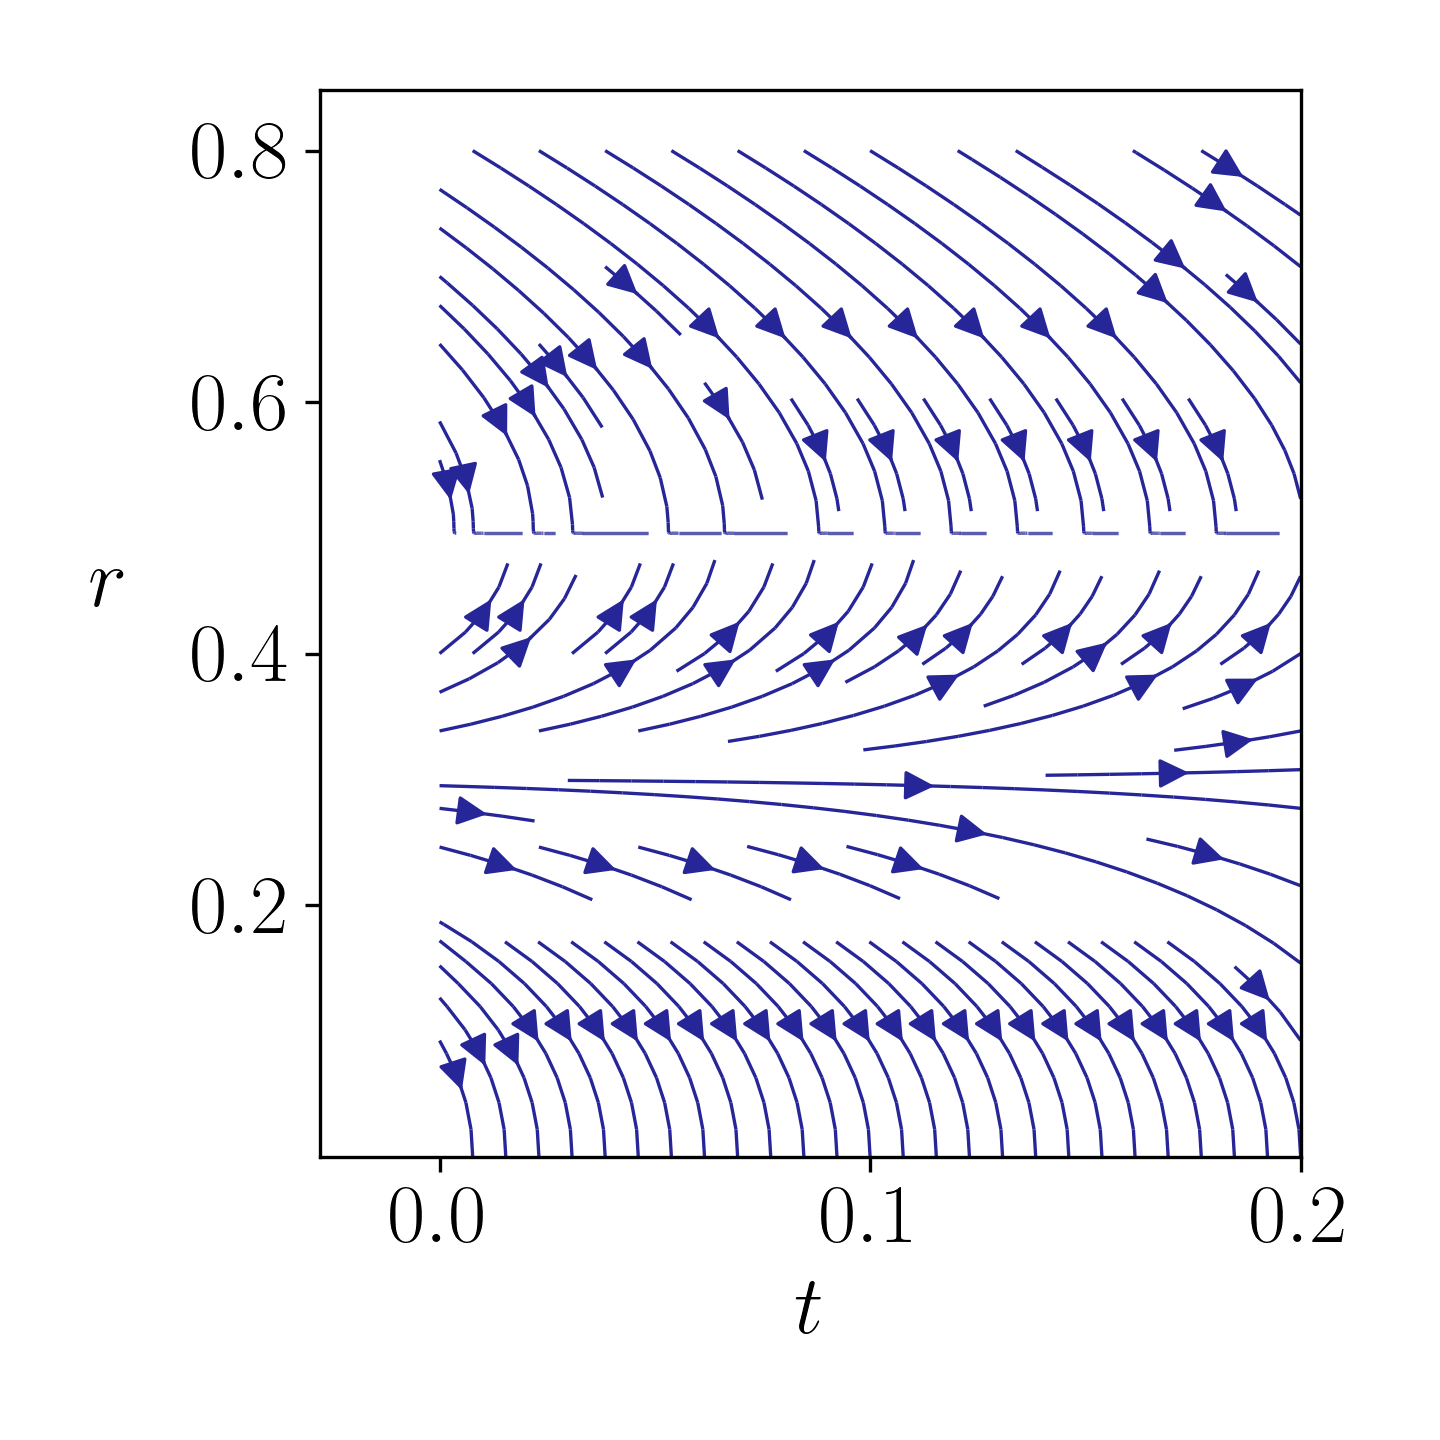
\includegraphics[width=\linewidth]{figures/streamlines/mod2-a40.png}
        \caption{$\alpha=0.4$}
        \label{fig:inverse-sub1}
    \end{subfigure}%
    \begin{subfigure}{.5\linewidth}
        \centering
        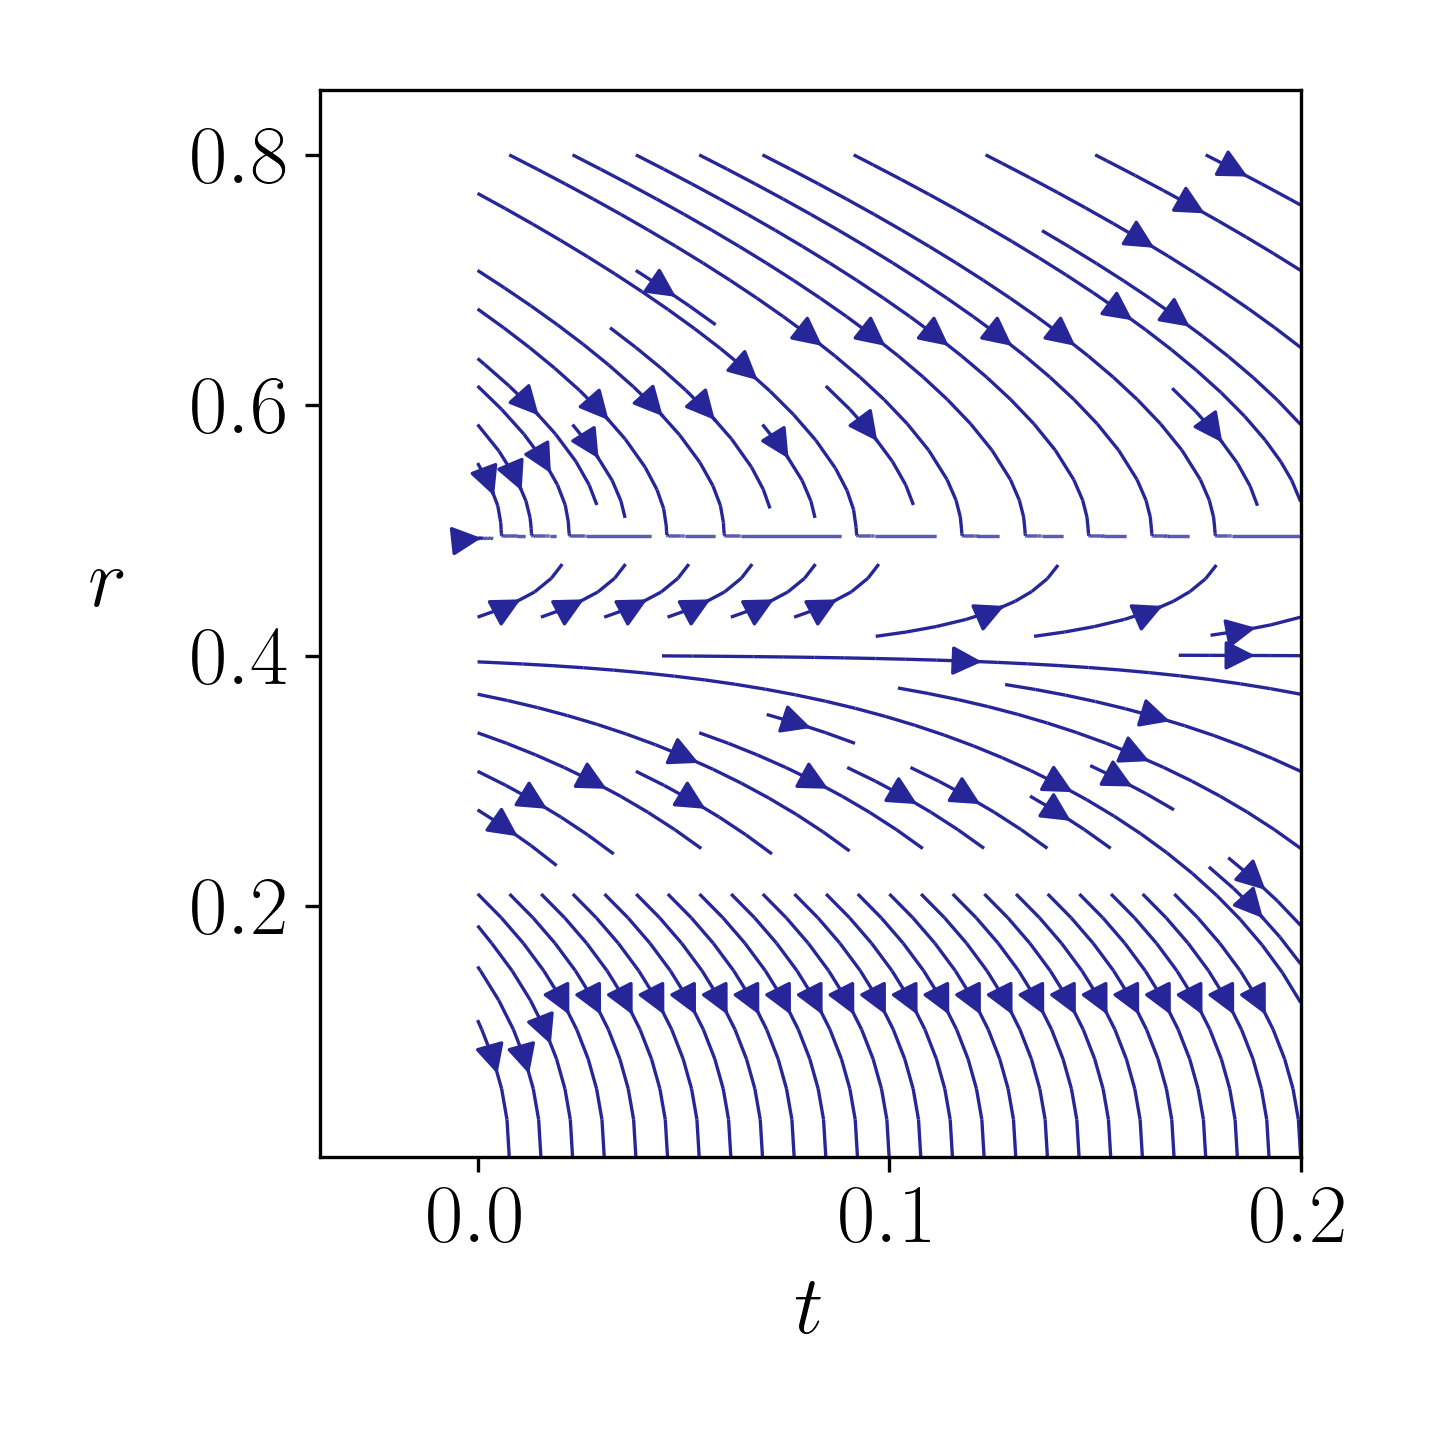
\includegraphics[width=\linewidth]{figures/streamlines/mod2-a20.png}
        \caption{$\alpha=0.2$}
        \label{fig:inverse-sub2}
    \end{subfigure}
    \caption[Streamlines for alternative velocity field]{Streamlines for the zero level set curve, $\Gamma(t)$, in the radially symmetric situation with the point set, \pointset, situated at $r_v=0.5$ and for the velocity field depending on the inverse distance \eqref{eq:general-inverse-velocityfield}.}
    \label{fig:total-streamline-inverse}
\end{figure}

Also, as we did above, we look at the streamlines for the zero level set curves starting at different initial radii in \figref{fig:total-streamline-inverse} for $\alpha=0.4$ and $\alpha=0.96$. Notice the difference in time scale from \figref{fig:total-streamline-picture} to \figref{fig:total-streamline-inverse}, where we see that the velocities are much grater when $r_{\Gamma}$ approaches $r_v$. It could also appear from \figref{fig:total-streamline-inverse} that we have a stable solution in $r_{\Gamma}=r_v$, but when inserting this into the equations for the curve velocity $r_v$ in \eqref{eq:pde-zero-streamline-inverse-1} and \eqref{eq:pde-zero-streamline-inverse-2}, we get

\begin{alignat}{3}
    r_t &= -&\bigg(\frac{\alpha}{\delta} + \frac{(1-\alpha)}{r_v}\bigg) \quad &\text{for }r(t) = r_{\Gamma}\geq r_v, \label{eq:pde-streamline-inverse-1}\\
    r_t &= &\bigg(\frac{\alpha}{\delta} -  \frac{(1-\alpha)}{r_v}\bigg) \quad &\text{for }r(t) = r_{\Gamma}<r_v,\label{eq:pde-streamline-inverse-2}
\end{alignat}
which is non-zero for $\delta \neq (\alpha r_v)/(1-\alpha)$. We thus have observed a discontinuity in the velocity function at $r=r_v$, where the velocity is very high in opposite directions slightly inwards or outwards of the point set radius, $r_v$. This will mean that if we solve this equation numerically, we will observe oscillations around the radius of the point set.

This oscillating behavior is very important to notice, because as we now have seen, there is no guarantee that we will obtain a stationary solution for all configurations of point sets. In order to obtain a stationary solution, a specific relation between curvature and distance must be fulfilled, and we see now that if the points are too densely spaced, there is not enough space to obtain the high curvature needed to balance the distance function.

In fact solving \eqref{eq:model2-pde} with $u_t=0$ for the curvature, yields a distance-curvature relation where the sign is decided by $\sigma$ locally: 
\begin{equation}
    \kappa (u) = \pm \frac{\alpha}{(1-\alpha)(\beta \distanceVm+\delta)}.
    \label{eq:dist-curv-relation-m2}
\end{equation}
From this, we see that in order to satisfy this, the curvature will be high close to the points and further and further away from the points, the curvature will decrease and yield straighter and straighter curves.

Further more, we can for model 2 not make a similar streamline picture as \figref{fig:total-streamline-picture} where we view the streamlines for all level curves given an initial radius for the zero level curve. For model 1, we got that the sign only changed once and the time of the sign change could be calculated, but for model 2, the sign will change infinitely fast and infinitely many times. 

We thus do not get as much information about model 2 for this radially symmetric situation. But this is an interesting result as well, because we have seen that not all point sets for all models yield a stationary solution at all. We have here seen that the zero level curve will stop at the point set for the provided example, but the requirement that $r_t=0$ is not fulfilled.

\begin{comment}
\textit{What do I have to say in this section?}
\begin{enumerate}
    \item Curve stationary (oscillating) when covering the point set
    \item Straight lines between, high curvature close
    \item Oscillation, and high velocities close to points
    \item $\kappa(u)=-\frac{\alpha}{1-\alpha} 1/(d+\delta)$.
\end{enumerate}
\end{comment}

\section{Model 3} 
As we just have seen, model 2 is constructed to have high curvature close to the sampled points only bounded by the small parameter $\delta>0$. The idea for the third model is to still have an inverse relation to the distance, but to bound the curvature in a more controlled way. It was Samson Seifu, a PhD student in our team who proposed the idea of the new distance dependent function, namely
\begin{equation*}
    f_3(d(\mathbf{x}; V)) = \frac{\sigma(\mathbf{x},t)}{\pi/2}\arctan(1/(\beta d(\mathbf{x}; V)))
\end{equation*} 
When $d\to 0$, $f_3(d) \to 1$, and thus there is no need for the parameter $\delta$ to avoid a singularity. The resulting model is thus

\begin{tcolorbox}[title=Model 3]
\begin{equation}
    u_t = |\nabla u| \bigg[ \frac{\alpha \sigma(\mathbf{x}, t)}{\pi/2} \tan^{-1}\bigg(\frac{1}{\beta \distanceVm}\bigg) + (1-\alpha)\kappa (u) \bigg], \quad \alpha, \beta \in \realspacem
    \label{eq:model3-pde}
\end{equation}
\end{tcolorbox}

Again, we do the same analysis on the radially symmetric example in order to get a feeling of how the curve, \curve\, will move following this model.

\subsection{Radially Symmetric Analysis}
We proceed in the in the same manner as for the two previous models. We rewrite the equation from $u(x, y)\to u(r)$ using \eqref{eq:curvature-circle} and \eqref{eq:nablau-ur}.
\begin{equation}
    u_t = u_r \, \bigg( \frac{\alpha \sigma(r, t)}{\pi/2} \tan^{-1}\bigg(\frac{1}{\beta |r-r_v|} \bigg) + \frac{1-\alpha}{r} \bigg).
    \label{eq:model3-rad}
\end{equation}
We can perform the same derivation as for model 1 and 2, deriving the ODE for the characteristics for the zero level curve, \curve:
\begin{equation}
    r_t = \frac{\alpha}{\pi/2} \tan^{-1}\bigg( \frac{1}{\beta(r(t)-r_v)}\bigg) + \frac{1-\alpha}{r(t)} \qquad \text{for } r(t)=\radgammam.
    \label{eq:model3-streamline-zero-levelcurve}
\end{equation}
Using \eqref{eq:sigma-radius-1} and \eqref{eq:sigma-radius-2} for the sign function $\sigma(r, t)$, we get the ODEs for all level curves:
\begin{alignat}{3}
    &r_t = - &(\alpha \tan^{-1}\big(\frac{1}{\beta|r(t)-r_v|} \big) + \frac{1-\alpha}{r(t)})  \qquad \text{when }&\radgammam\geq r_v, \\
    &r_t =  &(\alpha \tan^{-1}\big(\frac{1}{\beta|r(t)-r_v|} \big) - \frac{1-\alpha}{r(t)})  \qquad \text{when } &\radgammam< r_v.
\end{alignat}

Examples of such curves can be viewed in \figref{fig:total-streamline-arctan}. This shows the streamlines for zero level curves stemming from different initial radii. Here we can see that compared to model 2, the velocity near the point set is not as big, but increasing the value of $\beta$ yields a more similar shape for the streamline compared to model 2. However, since $\lim_{x\to\infty}\frac{2}{\pi} \arctan (x)=1$, the velocity will not be as high close to the sample points as model 1 with a small parameter $\delta$. 

\begin{figure}
    \begin{subfigure}{.5\linewidth}
        \centering
        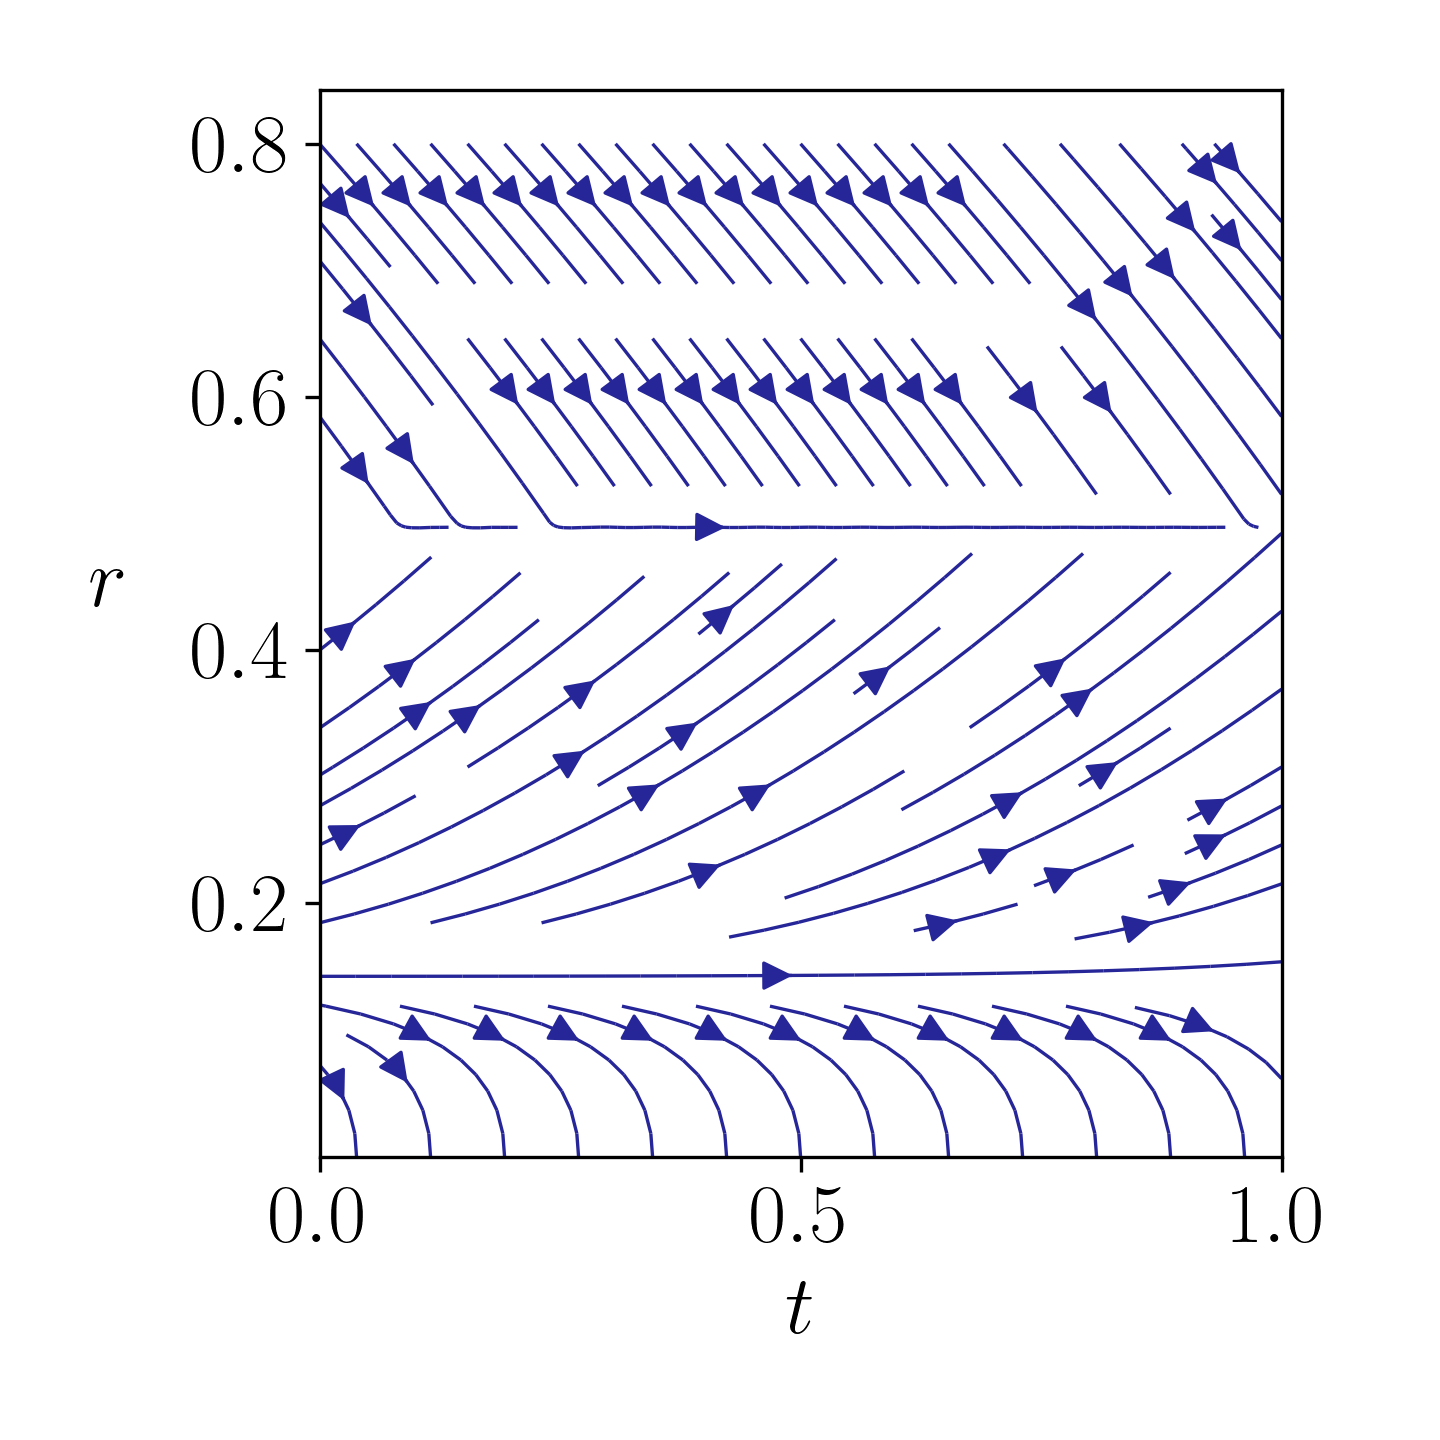
\includegraphics[width=\linewidth]{figures/streamlines/mod3-a90.png}
        \caption{$\beta=1$}
        \label{fig:arctan-sub1}
    \end{subfigure}%
    \begin{subfigure}{.5\linewidth}
        \centering
        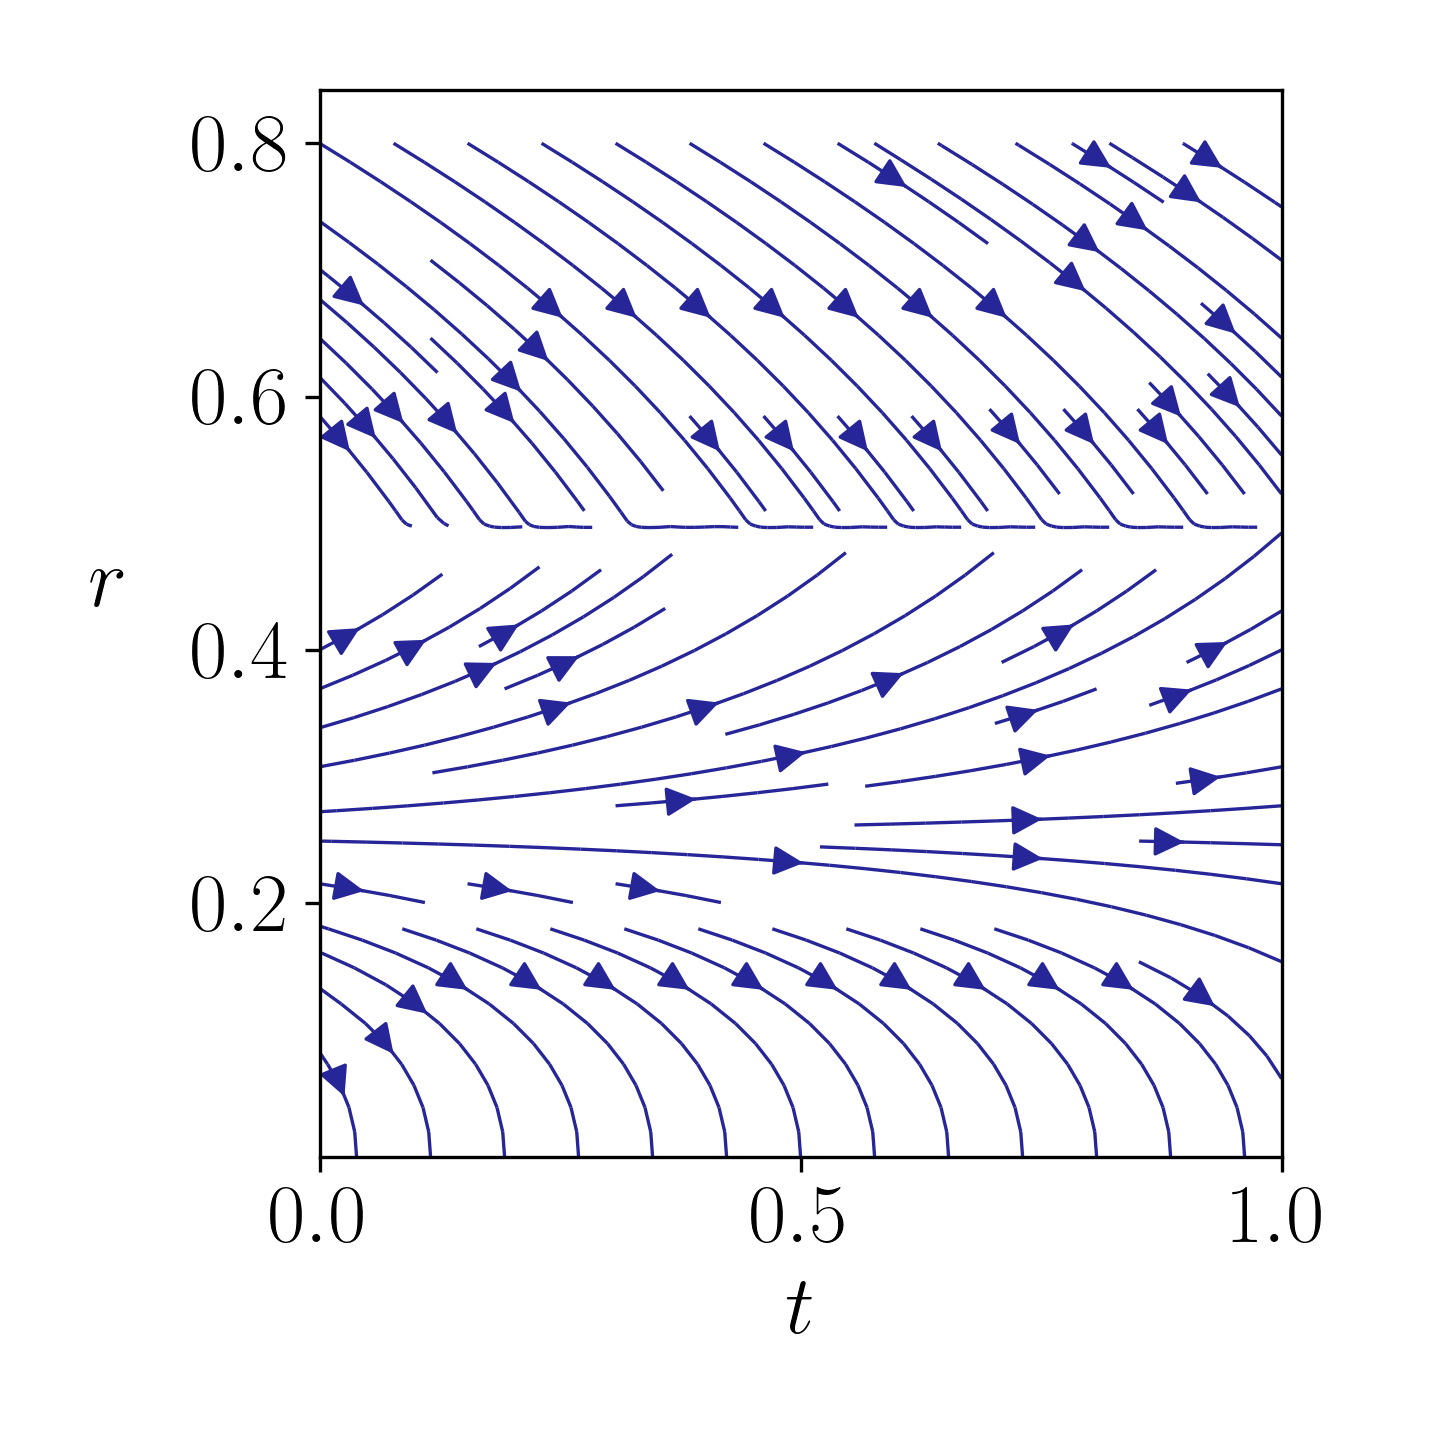
\includegraphics[width=\linewidth]{figures/streamlines/mod3-a90-b5.png}
        \caption{$\beta=5$}
        \label{fig:arctan-sub2}
    \end{subfigure}
    \caption[Streamlines for model 3]{Streamlines for the zero level set curve, $\Gamma(t)$, in the radially symmetric situation for model 3 defined in \eqref{eq:model3-pde} with the point set, \pointset, situated at $r_v=0.5$ and with parameter $\alpha=0.9$.}
    \label{fig:total-streamline-arctan}
\end{figure}

We move on to stationary solutions. As before, we are only interested in stationary solutions for the zero level curve, so we set $r_t$ from \eqref{eq:model3-streamline-zero-levelcurve} equal to zero.
We denote the stationary radius as $r_f$ and get \todo{Hva gjør jeg med dette???}
\begin{equation*}
    0 = \alpha \tan^{-1}\bigg( \frac{1}{\beta(r_f-r_v)} \bigg) + \frac{1-\alpha}{r_f}.
\end{equation*} 
\begin{comment}
After some simple operations, we obtain an implicit solution for the stationary radius,
\begin{equation}
    r_f-r_v = \bigg( \tan \bigg(\frac{1-\alpha}{\alpha r_f}\bigg) \bigg).
\end{equation}


\begin{enumerate}
    \item Curve stationary when covering the point set.
    \item Straight lines between, higher curvature close to points
    \item $\kappa(u) = \frac{\alpha}{1-\alpha} 2/\pi \arctan(1/d)$
\end{enumerate}
\end{comment}
\clearpage



\clearpage